%\boldmath
Widespread adoption of smartphones and tablets has enabled people to multiplex their physical reality, where they engage in face-to-face social interaction, with Web-based social networks and apps, whilst emerging 3D Web technologies hold promise for networks of parallel 3D virtual environments to emerge. Although current technologies allow this multiplexing of physical reality and 2D Web, in a situation called PolySocial Reality, the same cannot yet be achieved with 3D content. Cross Reality was proposed to address this issue; however so far it has focused on the use of fixed links between physical and virtual environments in closed lab settings, limiting investigation of the explorative and social aspects. This paper presents an architecture and implementation that addresses these shortcomings using a tablet computer and the Pangolin virtual world viewer to provide a mobile interface to a corresponding 3D virtual environment. Motivation for this project stemmed from a desire to enable students to interact with existing virtual reconstructions of cultural heritage sites in tandem with exploration of the corresponding real locations, avoiding the adverse temporal separation caused otherwise by interacting with the virtual content only within the classroom. The accuracy of GPS tracking emerged as a constraint on this style of interaction.

\section{Introduction}
The rapid adoption of smartphones and tablets and their popularity for social interaction via the mobile Web~\cite{Accenture2012} has led to people increasingly mixing their online and `real life' behaviours, multiplexing traditional face-to-face social interaction with Web-based social networks and apps. The pervasive provision of these devices provides a new mechanism for people to take physical space for granted, to cerebrally occupy a Web-based location whilst their bodies are simultaneously established in a physical location~\cite{Applin2011}. The term PolySocial Reality (PoSR) has been proposed to describe these multiplexed mixed realities~\cite{Applin2011a}, wherein individuals interact within multiple environments~\cite{Applin2012}, and to identify the extent and impact of shared and unshared experience in such situations~\cite{Applin2012a}. Whilst current technologies allow PoSR involving 2D Web content to manifest, attempting the same with 3D content is marred by the `vacancy problem': the inability to immerse oneself in 3D content whilst maintaining awareness of one's physical surroundings~\cite{Lifton2007a}, or put another way the inability to simultaneously experience a sense of presence in both grounded and synthetic realities. With the majority of players of popular Massively Multiplayer Online games (MMOs) wishing they could spend more time playing, over a fifth even wanting to spend all of their time in game~\cite{Castronova2006}, and with social roles and the community aspect constituting key aspects of these game's popularity~\cite{Castronova2006, Bartle2004}, exploring approaches for achieving 3D PoSR is prudent as demand for access to 3D social environments will only increase as 3D Web technologies further develop and more increasingly appeal to general social Web users and to educators in addition to gamers.

The capacity of 3D environments to provide extensible collaborative platforms for the reconstruction of cultural heritage sites and the potential of such reconstructions to promote understanding of and engagement with cultural heritage content both in public and classroom settings has been demonstrated~\cite{Allison2012,Kennedy2012}. This research tested various deployment scenarios, leveraging different control methodologies (traditional keyboard and mouse, Xbox controllers and gesture recognition via Kinect) and display options (regular 24'' desktop monitors, larger 40'' televisions and still larger 150'' projection) along with voice interaction with actors playing the parts of historical figures. These scenarios support three deployment modes; a network of reconstructions accessible via the Internet as part of the OpenSim hypergrid; portable LAN exhibitions where multiple computers are connected to a server via local network suitable for classroom use; and immersive installations combining projection and Kinect for use in museums and cultural heritage centers. In all these scenarios a recurrent theme has been the relationship between the virtual reconstruction and the physicality of the corresponding physical site. Frequently projects have involved interactions with the reconstruction and subsequent visits and tours of the physical site; however the temporal separation between these activities makes it harder to appreciate the sometimes complex relationships between the two. To overcome this temporal separation of experiencing the virtual and the real it is necessary for the virtual representation to be accessible in tandem at the physical site by overcoming the vacancy problem.

The cross reality concept~\cite{Lifton2007a, Paradiso2009} was proposed as an approach to address the vacancy problem and describes the mixed reality situation that arises from the combination of physical reality with a complete~\cite{lifton:merging} 3D virtual environment. Previous cross reality experiments did not address the explorative nor social elements of the paradigm as they focused on static locations at which the two environments were linked within closed lab surroundings~\cite{Applin2011}. The project described in this paper addressed these omissions with the Pangolin virtual world viewer~\cite{Daviesa} that uses a tablet computer with location and orientation sensors to provide users with a mobile cross reality interface allowing them to interact with 3D reconstructions of cultural heritage sites whilst simultaneously exploring the corresponding physical site, providing a sense of presence at both the physical site and in the reconstruction. The primary difference between this style of interaction and the more widely explored Augmented Reality (AR) concept is that cross reality concerns systems in which the virtual content constitutes a complete environment, as opposed to the sparse and discrete objects that AR positions upon a view of the real environment. This allows the virtual environment of cross reality systems to be accessed in absence of the real environment and allows for more encompassing graphical content.

\section{Scope}
The amount that the real and virtual environments that constitute a cross reality system spatially relate to each other is an important design decision which largely prescribes the style of interaction of the system as a whole. If the two environments have a high degree of spatial equivalence, that is to say that even if their visual appearances differ substantially that their fundamental layout and dimensions are the same such that navigating freely in one will never result in a collision with an object in the other (an allusion to the `mirror world' concept~\cite{Gelernter1993, Bar-Zeev2007, Roush2007}), then monitoring a user's movements within the real environment provides a method for controlling their avatar within the virtual environment without the need for concious manual control. This approach substantially lightens the cognitive load of maintaining a presence in a virtual environment, which is one of the main contributors to the vacancy problem.

This paper presents a cross reality project in which there is a high degree of spatial equivalence between the real and virtual environments, as it deals with bringing together virtual reconstructions of cultural heritage sites with their corresponding real locations. The backdrop for many of the experiments is the impressive ruins of the St Andrews cathedral, while the virtual environment is a `distorted'~\cite{lifton:merging} OpenSim simulation of the same location that presents a historically accurate reconstruction of the cathedral as it would have stood at the peak of its former glory~\cite{Kennedy2012, OpenVirtualWorldsgroupSchoolofComputerScience} (see figure \ref{cathedral_picture}). This is a large reconstruction, over 400m by 600m, of a complex multi-storey building and thus represents a challenge for a mobile device to render and consequently is considered a good platform for testing.

\begin{figure}[h]
\centering
\includegraphics[width=0.48\textwidth]{images/figure_1}
\caption{OpenSim reconstruction of the St Andrews cathedral.}
\label{cathedral_picture}
\end{figure}

The same pioneering collaborations between computer scientists, educationalists and historians that led to the creation of the St Andrews cathedral reconstruction have also led to the creation of reconstructions of; a 6th Century Spartan Basilica, Virtual Harlem (1921), Linlithgow Palace (1561), Brora Salt Pans (1599), Featherstone Fishing Station (19th century), Eyemouth Fort (1610), an Iron Age Wheel House and Caen Township (1815). These reconstructions provide a platform for interactive historical narratives, a stage for visitors to play upon and engage in both serious (and not so serious) games both alone and with other users, and serve as a focal point for educational investigations into local history and culture [9, 18]. The reconstructions have been widely used in a range of real world educational contexts. In the formal sector they have been a vehicle for investigative research, part of degree accredited university modules and used in both primary and secondary education. They have also been used as the content for interactive museum installations, art installations and community groups. This has involved further collaborations with Education Scotland, Historic Scotland, SCAPE Trust, Timespan cultural center, the Museum of the University of St Andrews (MUSA), Madras College, Linlithgow Palace and Strathkiness Primary School.

The project described in this paper furthers this previous work by developing a mobile interface to allow students to explore both a physical site and its virtual reconstruction in tandem, rather than having to explore the reconstruction from a computer in the classroom and trying to relate what they had seen to a visit to the physical site at a later date. Figure \ref{separation_map} shows how small the spatial separation between the classroom and the physical site was during a session with students at St Andrews' Madras College. This project, introduced in~\cite{Davies2012}, developed a modified version of the Second Life viewer called Pangolin, which through use of sensors allows movement of the avatar and camera to be implicitly controlled by sensing the physical position and orientation of the tablet computer which the user carries and upon which the viewer executes. Figure \ref{pangolin_in_action} depicts the system in use at the St Andrews cathedral.

\begin{figure}[h]
\centering
\includegraphics[width=0.48\textwidth]{images/separation_map}
\caption{Aerial photograph of St Andrews demonstrating the distance between Madras College (left ring) and the cathedral itself (right ring). The distance between the two sites is roughly 650m, with the photograph being approximately 1km across.}
\label{separation_map}
\end{figure}

\begin{figure}[h]
\centering
\includegraphics[width=0.48\textwidth]{images/figure_3}
\caption{The Pangolin viewer running on a tablet computer at the St Andrews cathedral, with the camera orientation of the viewer synchronised to the physical orientation of the tablet, the view of the virtual reconstruction corresponding to that of the physical ruins.}
\label{pangolin_in_action}
\end{figure}

This system promises to augment exploration of cultural heritage sites by allowing convenient navigation of the 3D reconstruction and stimulating reflection through the close juxtaposition of the remains and an accessible interpretation. The use of a complete virtual environment also allows for the possibility of interaction between individuals and groups at the site with remote participants, including domain experts, who are connected to the reconstruction from a distant physical location.

\section{Methods}
\subsection{Virtual Environment}
The 3D virtual environment component of the Pangolin system was implemented using the Second Life/OpenSimulator (SL/OpenSim) platform, which provides a 3D social-oriented multi-user non-competitive virtual environment which focuses on the community, creation and commerce~\cite{Sevan2008} aspects of many users interacting within a shared space through the abstraction of avatars, rather than the competitive natures of games and the solitary environments commonly afforded by simulation and visualization platforms. The distributed client/server model of SL/OpenSim, wherein 3D content is stored on a grid of servers operated by a multitude of organizations and distributed to and navigated between by dispersed clients on demand when they enter a particular region rather than being pre-distributed as is the norm for games, simulations and visualizations, is analogous to the manner in which 2D social Web content is served from Web servers to client browsers and apps. This style of content delivery is necessary when considering the dynamic and ephemeral nature of consumer-generated media which constitutes the majority of the current 2D social Web and will make up the majority of expanding 3D social Web content.

Whilst SL/OpenSim encapsulates many of the desirable architectural features for 3D PoSR experiments it does not support execution upon familiar mobile platforms (Android/iOS) nor does it provision for avatar control from sensor data. However the open source nature of the SL viewer allowed modifications to be effected, enabling control of the avatar and camera from real time data collected from position and orientation sensors connected to a tablet computer. This ability to control navigation within the 3D virtual environment without explicit conscious input of keyboard/mouse/touch commands is integral to reducing the cognitive load required to maintain a presence within a virtual environment which is a key requirement for overcoming the vacancy problem and achieving successful mobile cross reality.

As the SL viewer is only available for x86 platforms the choice of user hardware platform for the experiments was limited, with the MSI WindPad 110W presenting the most promising solution: a 10'' tablet computer sporting an AMD Brazos Z01 APU (combining a dual-core x86 CPU and Radeon HD6250 GPU)~\cite{Micro-StarInt'lCo.}. The user's position was monitored using GPS, a solution which is well suited to applications of the system within the use case of cultural heritage; such sites often constitute outdoor ruins at which a clear view of the sky allows for good GPS connectivity. For use cases where a similar modality of interaction is desired whilst indoors then an indoor positioning system would be used; a roundup of such technologies is available in~\cite{Mautz2012}.

To reduce computational load on the 110W, the OpenSim server was run on a separate Lenovo ThinkPad X61s laptop computer during the experiments. Due to the limited range of the laptop's wireless interface, the laptop was connected by RJ45 ethernet cable to a Linksys WRT54G wireless router to allow the 110W to access the OpenSim server wirelessly from anywhere within the experiment area. The router was powered from a 12V sealed lead-acid battery. This setup is shown in figure \ref{server}.

\begin{figure}[h]
\centering
\includegraphics[width=0.48\textwidth]{images/server}
\caption{Lenovo ThinkPad X61s laptop, Linksys WRT54G wireless router and sealed lead-acid battery providing OpenSim server via wireless to the 110W.}
\label{server}
\end{figure}

\subsection{GPS Configuration}
The 110W features an AzureWave GPS-M16~\cite{AzureWave} GPS receiver; however poor API provision and meager documentation lead to use of a separate u-blox MAX-6 GPS receiver~\cite{U-bloxAG} outfitted with a Sarantel SL-1202 passive antenna~\cite{Sarantel}. The MAX-6 is of higher operational specification than the GPS-M16 and supports Satellite Based Augmentation Systems (SBAS) which improve the accuracy of location data by applying additional correction data received from networks of satellites and ground-based transmitters separate to those of the GPS system. These networks include the European Geostationary Navigation Overlay Service (EGNOS) that covers the UK where the experiments took place.

The product summary for the MAX-6 claims accuracy of 2.5m Circular Error Probable (CEP) without SBAS corrections and 2m CEP with SBAS corrections ``demonstrated with a good active antenna''~\cite{U-bloxAG2012}. This means that, in an ideal situation with SBAS correction data available, there would be 50\% certainty that each position reported by the GPS receiver would be within 2m of its actual position. The SL-1202 antenna used is passive, however as the distance between antenna and the MAX-6 IC itself in the hardware application is only a few millimeters there would have been negligible benefit from using an active antenna. However whether the SL-1202 constitutes `good' for achieving the headlining performance characteristics of the MAX-6 is debatable as the definition of `good' was not provided in the product summary.

The MAX-6 was operated in `pedestrian' dynamic platform model, use of SBAS correction data was enabled and frequency of readings was set to the maximum of 5Hz.

To determine the real world accuracy attainable with the MAX-6 outfitted with the SL-1202 in situations akin to those of the cultural heritage case study, a walking route around the St Andrews cathedral ruins, akin to the route that an individual visitor or school group might take, was planned and then walked with the MAX-6 connected to a laptop computer via an Arduino operating as a Universal Asynchronous Receiver/Transmitter (UART) feeding the raw National Marine Electronics Association (NMEA) messages into the `u-center'GPS evaluation software version 7.0 which logged the messages for later evaluation. Simultaneously for comparative purposes a mid-range consumer Android smartphone was used to record the same track; a HTC One S~\cite{HTCCorporation2013} containing a gpsOne Gen 8A solution within its Qualcomm Snapdragon S4 processor~\cite{QualcommIncorporated2013} and using Google's `My Tracks' app version 2.0.3 to record the data. The three sets of positional data (planned route, MAX-6 recorded route and smartphone recorded route) were entered into a PostgreSQL database~\cite{Daviesc,Daviesb} and the PostGIS database extender's ST\_HausdorffDistance algorithm~\cite{PostGIS} was used to calculate the Hausdorff distances between the recorded routes and the planned route and between the recorded routes themselves. In this scenario, the Hausdorff distance represents the furthest distance needed to travel from any point on the route recorded by the GPS receiver to reach the nearest point on the planned route. Because of the substantially greater inaccuracies identified in the latter part of the recorded tracks, separate Hausdorff distances were calculated both for the complete tracks and also for truncated first and second sub-tracks.

\subsection{GPS to OpenSim conversion}
Translating real world positions, obtained via the GPS receiver as latitude and longitude pairs, into corresponding OpenSim (X,Y) region coordinates is achieved using the haversine formula~\cite{Gellert1989} from spherical trigonometry. The prerequisites for this approach are that the OpenSim model is aligned correctly to the OpenSim compass as the real location is aligned to real bearings (although provision to specify an `offset' within the Pangolin viewer for non-aligned models would be a trivial addition), that the model was created to a known and consistent scale and that a single `anchor point' is known for which both the real world latitude/longitude and corresponding OpenSim (X,Y) region coordinates are known.

Using the haversine formula the great-circle (or orthodromic) distance between the latitude of the anchor point and the latitude of the new GPS reading is calculated, then applying the scale of the model results in the equivalent distance in OpenSim metrics between the Y coordinate of the anchor point and the Y coordinate of the position corresponding to the new GPS reading. Repeating the same calculations with the longitude of the new GPS reading provides the distance between the X coordinate of the anchor point and the X coordinate of the position corresponding to the new GPS reading. Adding or subtracting these distances as appropriate to the OpenSim coordinates of the anchor point provides the OpenSim coordinates that correspond to the new GPS reading, to which the avatar is then instructed to move.

The anchor point is specified using global coordinates, not local coordinates. This allows navigation to operate across region boundaries and within mega regions (it is not limited to a single 256x256 meter OpenSim region) and there are no restrictions for the placement of the OpenSim component of the anchor point (it can be anywhere in any region, movement of the avatar can be in any direction from it (positive and negative), it does not have to be at the center of the model or even in a region that the model occupies).

Calculating a global coordinate is simply a case of multiplying the position of the region by 256 and then adding the local coordinate. For example, for an anchor at local coordinate $(127,203,23)$ within a region that is at $(1020,1042)$ the global X coordinate is calculated as $(1020 * 256) + 127 = 261247$ and the global Y coordinate as $(1043 * 256) + 203 = 267211$. Elevation (Z) is ignored due to a combination of the relatively low accuracy of these data attainable via GPS (when compared to the longitudinal/latitudinal accuracy) and as the case study explored involved users navigating outdoor ruins remaining at ground level.

\subsection{Orientation}
To control the SL camera in the required fashion, sensor data is collected for the direction that the user is facing (in terms of magnetic compass bearing) and the vertical angle (pitch) at which they are holding the tablet. Magnetic compass bearing is sensed using a magnetometer and pitch by an accelerometer. Roll data is also captured by the accelerometer, however it was expected that users would keep the tablet in a roughly horizontal fashion when interacting with it, thus using these data to control the SL camera's roll was not deemed to be beneficial and was not implemented.

The 110W does not feature a magnetometer and its tilt sensor is rudimentary (only useful for differentiating between discrete cases of landscape and portrait orientation for screen rotation). Several alternative sensors were auditioned, including the MMA8452, ADXL335, HMC5883L and eventually the HMC6343 which was adopted for the experiments. The HMC6343 combines a 3-axis magnetometer, 3-axis accelerometer and algorithms to internally apply the accelerometer's readings to tilt compensate the magnetometer's readings; tilt compensation is necessary for an accurate compass bearing when the device is not held in a perfectly level orientation, such as when the user tilts it up or down to view content above or below their eye level.

Magnetic declination information was entered into the HMC6343 for the position of the cathedral and the date of our experiments. The HMC6343's hard-iron offset calculation feature was used each time the hardware configuration was altered. The sampling frequency of the HMC6343 was set to its highest value of 10Hz. Orientation was set to `upright front' to match the physical orientation of the IC in the experiments.

\subsection{Interfacing GPS/Orientation hardware with SL}
The MAX-6 and HMC6343 were connected to an Arduino (the setup used throughout the experiments is shown in figure \ref{arduino}) and a `sketch' (the name given to programs that execute upon the Arduino platform) written to receive the data from the ICs, perform simple processing upon them and relay them to the tablet via USB connection~\cite{Davies}. The TinyGPS library~\cite{Hart} was used to abstract processing of NMEA messages from the MAX-6 to obtain the required latitude and longitude values.
 
\begin{figure}[h]
\centering
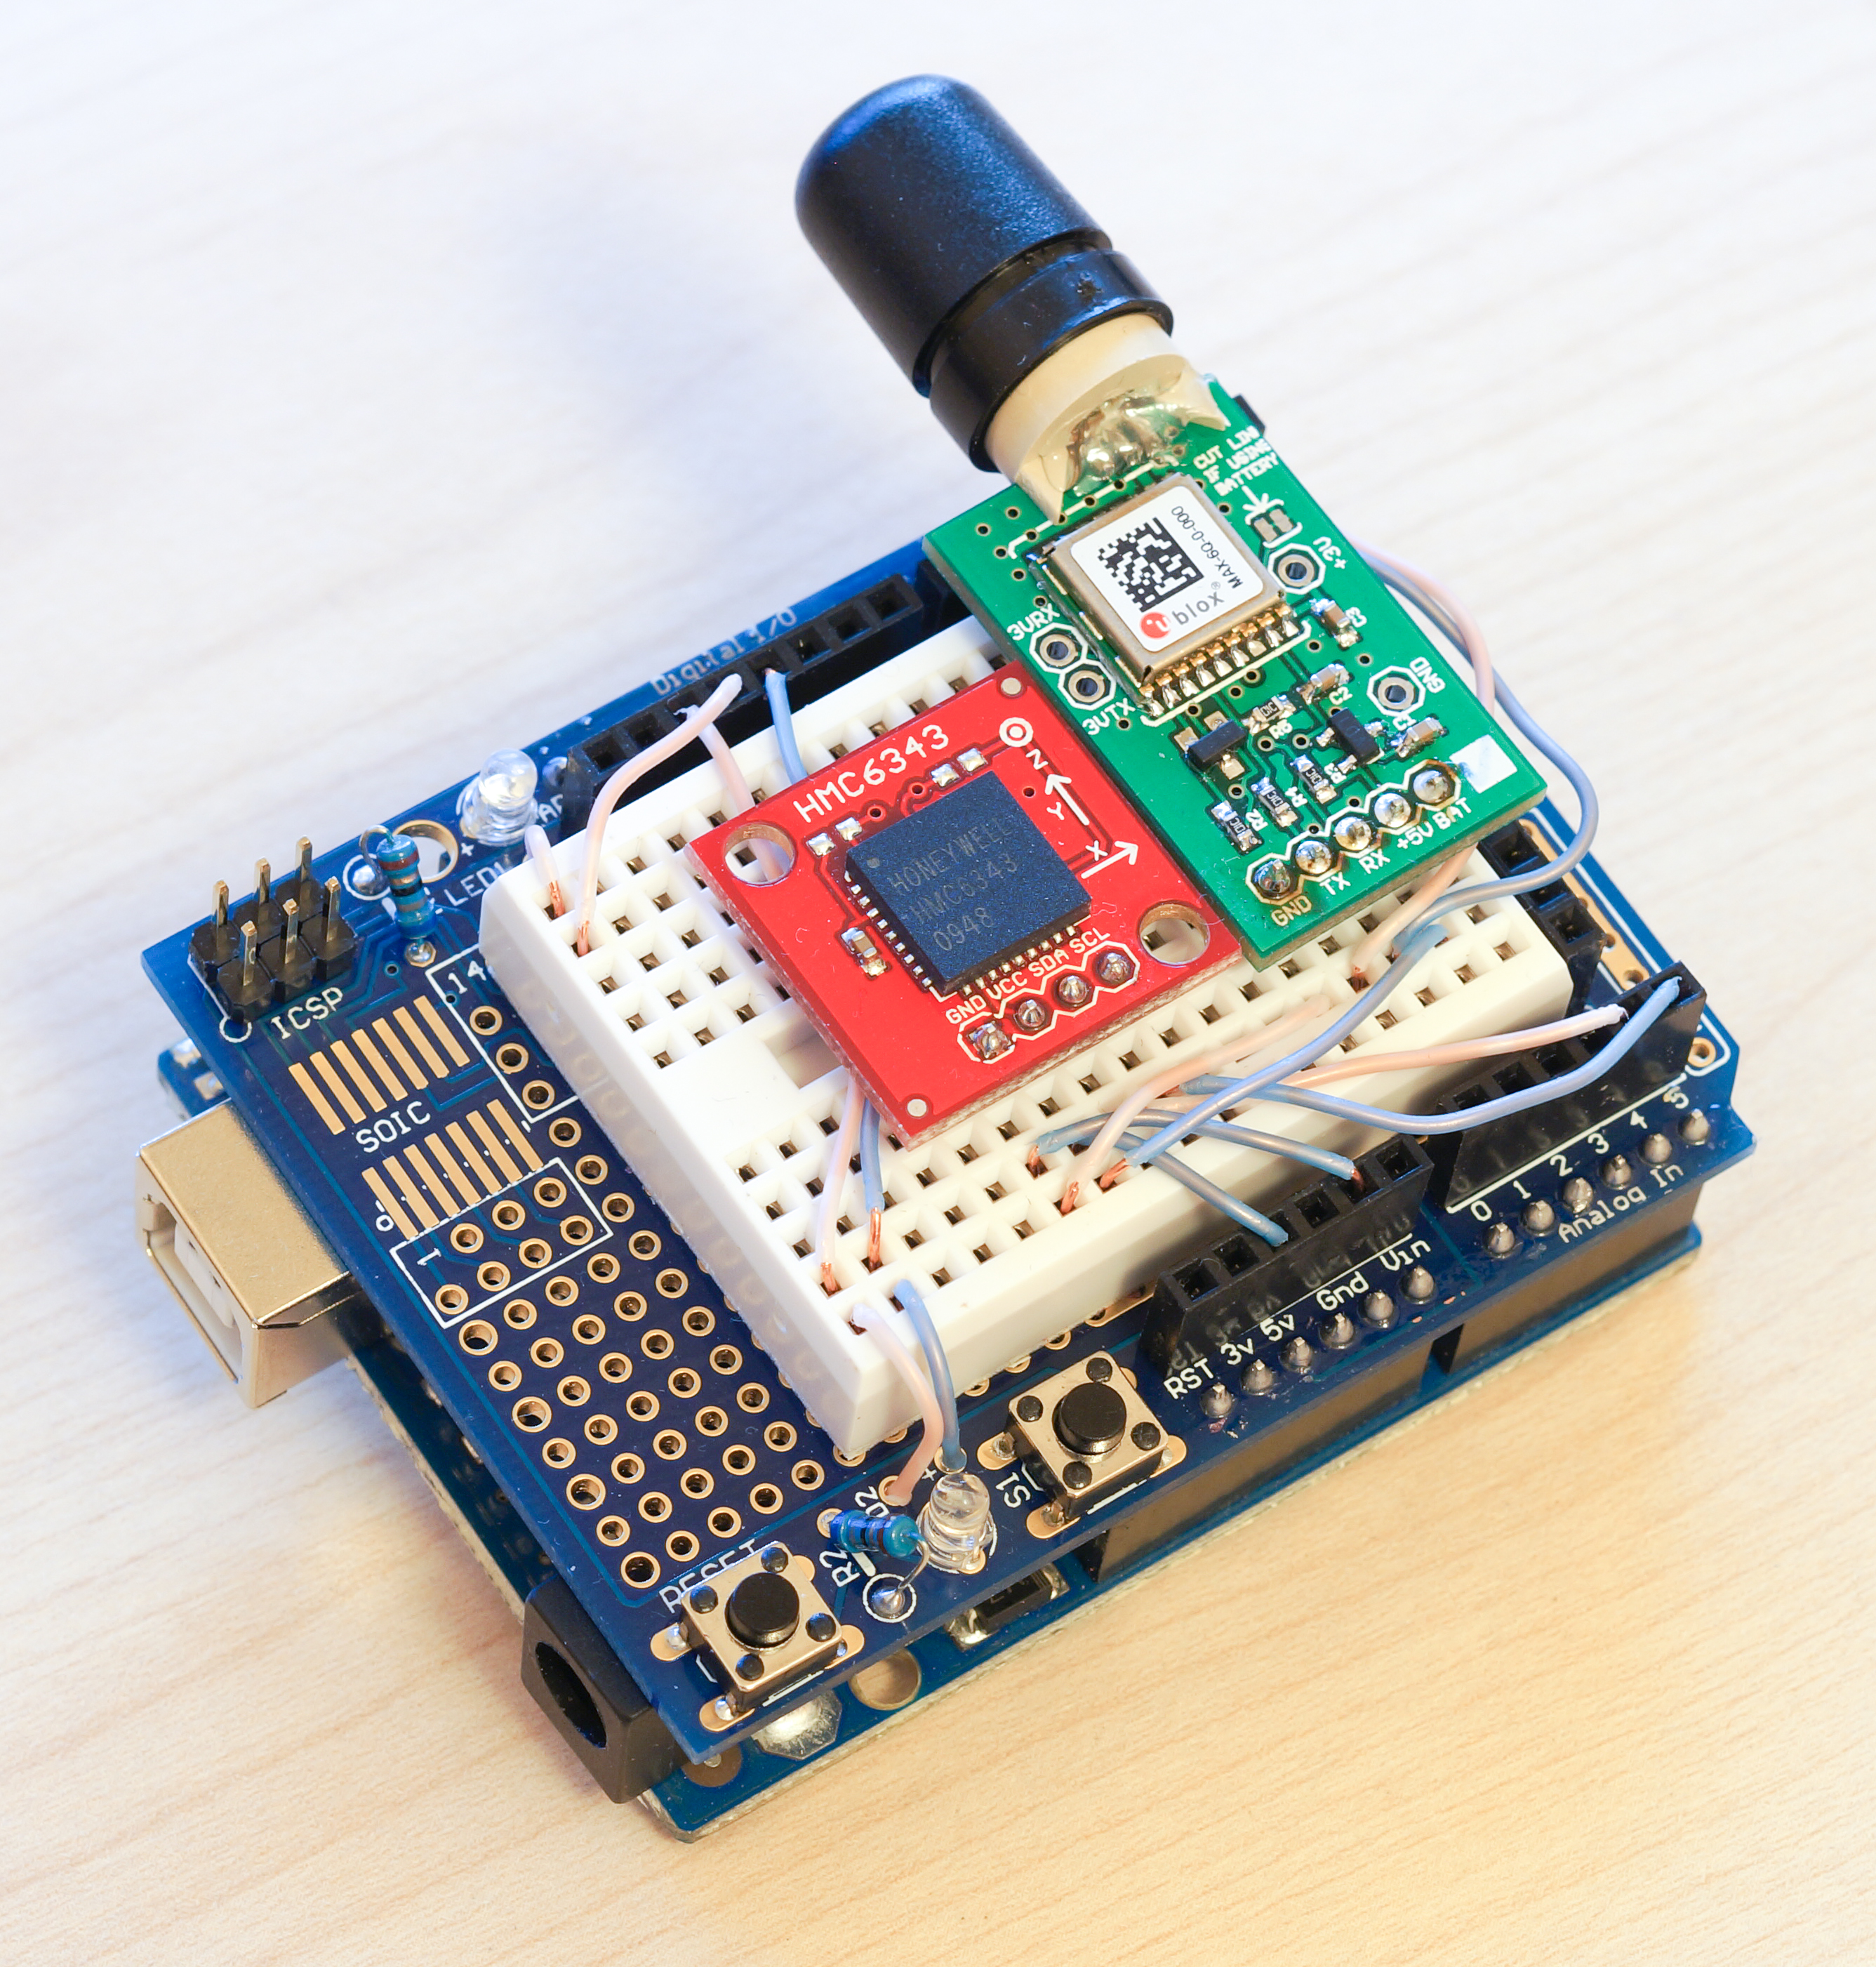
\includegraphics[width=0.48\textwidth]{images/figure_8}
\caption{The HMC6343, MAX-6 and SL-1202 connected via a breadboard prototyping shield to the Arduino, in the setup and configuration that was then attached to the rear of the 110W for the experiments.}
\label{arduino}
\end{figure}

\begin{figure}[h]
\centering
\includegraphics[width=0.48\textwidth]{images/tablet_back}
\caption{The setup from figure \ref{arduino} attached to the rear of the 110W. The sensors are configured such that (in the orientation of this photograph) the X axis is positive pointing straight down, Y is positive pointing straight right and Z is positive pointing perpendicular out of the rear face of the tablet.}
\label{tablet_back}
\end{figure}

Leveraging standard SL avatar/camera control interfaces was explored by programming the Arduino to mimic a standard USB HID joystick via the Lightweight USB Framework for AVRs (LUFA), sending messages that the viewer interpreted as coming from a joystick and allowing the use of the standard joystick options. However the granularity of control attainable via this method was not sufficient and thus the viewer was modified (giving rise to the Pangolin viewer) to make use of the Boost.Asio C++ library to support receiving data via serial port and to use these data to control the movement of the avatar and camera by directly interfacing with the control functions at a lower level of abstraction. Receipt of messages is performed in an asynchronous non-blocking fashion, with the viewer's main loop processing the most recently received message in each iteration. Messages follow the format

$\langle bearing \rangle$ $\langle pitch \rangle$ $\langle roll \rangle$ $\langle latitude \rangle$ $\langle longitude \rangle$

The viewer's GUI was modified with the addition of a dialogue that allows the user to specify the path of the serial device, separately enable or disable sensor-driven camera and movement control, as well as providing numerous controls for fine-tuning its behavior, including the ability to specify high-pass filters for avatar movement and specify the smoothing applied to camera control. This GUI also presents the necessary fields for input of the anchor point details and fields for diagnostic output of the received information. Figure \ref{pangolin_screenshot} shows this GUI within the Pangolin viewer.

\begin{figure}[h]
\centering
\includegraphics[width=0.48\textwidth]{images/figure_9}
\caption{The GUI within the Pangolin viewer that allows administration of the position and orientation control of the avatar. In this screenshot Pangolin is connected to the Arduino and is receiving position and orientation data.}
\label{pangolin_screenshot}
\end{figure}

\section{Results}
Two plausible modalities of interaction were identified for this system, with each presenting different requirements with regards to accuracy of position tracking.

The first modality is one in which a number of locations that represent points of particular interest are identified. This is already a common practice at cultural heritage sites, with such locations often bearing signs or placards presenting text and/or images explaining what can be observed from the position. With Pangolin, when a user walks within a certain range of such a point, their avatar can be moved to the corresponding location within the reconstruction (and a sound played to alert the user to the fact that there is something of interest to observe) from which they can then move the tablet around them to examine their surroundings in the reconstruction. This modality is similar to audio tours employed by many museums and cultural heritage sites, but replaces the requirement to follow a static route or type in numbers of locations with the ability to freely navigate the real environment with access to additional information being triggered automatically once within the required range of a point of interest.

The second modality is one of free roaming exploration, in which the movements of the user's avatar within the reconstruction mimic the user's movements within the real world as closely as possible.
The first modality can be scaled to function with different accuracies of position tracking; as long as the distance between any two points of interest is at least as much as the worst case performance of the position tracking then distinguishing correctly between different points will always succeed. The second modality requires extremely accurate position tracking, arguably surpassing the capabilities of mainstream GPS technology even in ideal situations.

During the experiments the MAX-6 was unable to maintain reception of the additional correction data required for SBAS operation; when left stationary for several minutes reception was possible however subsequent movement of only a few meters at walking pace broke the connection. This reduced the theoretical maximum performance of the unit to 2.5m CEP, with observed performance being lower. Figure \ref{map_one} depicts an aerial view of the St Andrews cathedral ruins; the blue line represents the planned route, red the route recorded by the MAX-6 receiver and green the route recorded by the smartphone for comparative purposes, both while walking the planned route.

\begin{figure}[h]
\centering
\includegraphics[width=0.48\textwidth]{images/figure_4}
\caption{Aerial view oriented North upward of the St Andrews cathedral ruins; the blue line represents the planned route, red the route recorded by the MAX-6 and green the route recorded by the smartphone whilst walking the planned route.}
\label{map_one}
\end{figure}

The Hausdorff distance between the planned route and that recorded by the MAX-6 was $1.02e^{-04\circ}$. The `length' of a degree of latitude and a degree of longitude depends upon location upon the Earth; around the location of the St Andrews cathedral 1$^\circ$ of latitude is equivalent to 111347.95m and 1$^\circ$ of longitude to 61843.88m. Thus the Hausdorff distance of $1.02e^{-04\circ}$ can be visualized as $\pm11.3$m of North/South inaccuracy or $\pm6.3$m of East/West inaccuracy (or a combination of both N/S and E/W inaccuracy not exceeding a total displacement of $1.02e^{-04\circ}$ from the planned route).

The MAX-6 did achieve better performance than the smartphone, which recorded a Hausdorff distance of $1.33e^{-04\circ}$ ($\pm14.8$m N/S, $\pm8.2$m E/W). The Hausdorff distance between the routes logged by the MAX-6 and the smartphone was $1.14e^{-04\circ}$ ($\pm12.7$m N/S, $\pm7.0$m E/W), which represents a low correlation between the inaccuracies recorded by the two receivers even though they are of similar magnitudes from the planned route.

The maximum inaccuracies were recorded when walking along the South wall of the cathedral's nave. This wall is one of the most complete sections of the building with stonework reaching some 30ft above ground level and providing an effective obstruction to line-of-sight to half of the sky (and substantially impairing reception of signals from GPS satellites) when in close proximity to it. When considering just the sub-route shown in figure \ref{map_two}, which terminates before this wall begins to significantly obstruct view of the sky, the Hausdorff distances are notably smaller; the MAX-6 achieved a Hausdorff distance of $7.23e^{-05\circ}$ ($\pm8.05$m N/S, $\pm4.47$m E/W) throughout this sub-route, with the smartphone still behind with $8.99e^{-05\circ}$ ($\pm10.01$m N/S, $\pm5.56$m E/W). Again the Hausforff distance between the receivers showed low correlation between the inaccuracies, at $6.43e^{-05\circ}$ ($\pm7.12$m N/S, $\pm3.98$m E/W).
 
\begin{figure}[h]
\centering
\includegraphics[width=0.48\textwidth]{images/figure_5}
\caption{Aerial view oriented North upward of the St Andrews cathedral ruins; the blue line represents the first sub-route of the planned route, red the sub-route recorded by the MAX-6 and green the sub-route recorded by the smartphone whilst walking the first planned sub-route.}
\label{map_two}
\end{figure}

When analyzing the tracks in the vicinity of the nave (see figure \ref{map_three}) it is shown that although the MAX-6 outperformed the smartphone in terms of Hausdorff distance this relationship can be considered misleading as the smartphone track corresponded more closely in shape to the planned route even if it did stray further at its extreme. The discrepancy in the behavior of the two receivers in this situation is attributed to different implementations of dead-reckoning functionality between the receivers. Dead-reckoning is the process used when a GPS receiver loses reception of location data from satellites and extrapolates its position based upon a combination of the last received position data and the velocity of travel at the time of receiving these data.
 
\begin{figure}[h]
\centering
\includegraphics[width=0.48\textwidth]{images/figure_6}
\caption{Aerial view oriented North upward of the St Andrews cathedral ruins; the blue line represents the second sub-route of the planned route, red the sub-route recorded by the MAX-6 and green the sub-route recorded by the smartphone whilst walking the second planned sub-route.}
\label{map_three}
\end{figure}

Pangolin's camera control from orientation data does not have as stringent performance criteria as the movement control from position data. Unlike augmented reality where sparse virtual content is superimposed upon a view of a real environment and the virtual objects must be placed accurately in order for the effect to work well, cross reality presents a complete virtual environment that is viewed `separately' or side-by-side with the real environment and thus discrepancies between orientation of real and virtual environments have a less detrimental effect to the experience. Although the accuracy of the camera control during the experiments was reported as being sufficient, the speed at which the camera orientation moved to match physical orientation was reported as being too slow, resulting in having to wait for the display to `catch up' to changes in orientation. This is attributed to the 10Hz sampling rate of the orientation sensors which, particularly after readings are combined for smoothing purposes to reduce jerky movement, resulted in too infrequent orientation updates. Frame rates within Pangolin whilst navigating the route averaged between 15 and 20 frames per second with the viewer's `quality and speed' slider set to the `low' position.

The style of explorative interaction with virtual content that this system employs is more resilient to input lag and low frame rates than other scenarios of interaction with virtual content such as fast paced competitive video games including First Person Shooters (FPS) [20], but overall user experience would nonetheless be improved by a faster sampling of orientation data and a higher frame rate. Additionally it should be noted that the cathedral reconstruction was created with relatively powerful desktop computers in mind as the primary deployment platform and has not been optimized for use on less powerful mobile platforms such as Pangolin. Performance of Pangolin on a less graphically complex OpenSim region (Salt Pan 2 [17]), that also depicts a reconstruction of a cultural heritage site, was better at 20 to 25 frames per second at the `low' position and between 15 and 20 frames per second at `high' (see figure 7).

\begin{figure}[h]
\centering
\includegraphics[width=0.48\textwidth]{images/figure_7}
\caption{Plot of Pangolin's performance (measured in frames per second) against different graphical settings (selected via the `Quality and speed' slider of the viewer) in two positions within the Salt Pan 2 region.}
\label{framerate_graph}
\end{figure}

\section{Interpretations}
The positional accuracy of $1.02e^{-04\circ}$ attained by the MAX-6 is sufficient for the first modality of interaction (that of distinguishing and navigating between multiple points of interest). This value of $1.02e^{-04\circ}$ (analogous to a combination of $\pm11.3$m of North/South inaccuracy or $\pm6.3$m of East/West inaccuracy) represents a constraint on the granularity of the content; it is the minimum distance required between any two points of interest for them to be correctly differentiated between. This same value is not sufficient for the second modality of interaction (that of free roaming exploration with avatars mimicking their users' movements as closely as possible). This modality would require the use of additional position tracking techniques to improve accuracy to around 1m CEP (analogous to $8.98e^{-06\circ}$ latitude or $1.62e^{-05\circ}$ longitude around the location of the St Andrews cathedral).

Use of a GPS receiver that is lower performance than the MAX-6 used by Pangolin, but more common due to being of the calibre integrated into smartphones and tablets such as that used in the experiments, is still sufficient for the first modality but with a larger minimum distance required between any two points of interest. The Hausdorff distance of $1.33e^{-04\circ}$ recorded by the smartphone used in the experiments is analogous to $\pm14.8$m N/S or $\pm8.2$m E/W around the location of the cathedral.

Observed accuracy of the orientation tracking is sufficient for both modalities of interaction; the accuracy of orientation tracking required does not change with different positional accuracy and the accuracy of orientation attained in the experiments is sufficient for an acceptable user experience, however the experience would benefit from better graphical quality and higher responsiveness to changes in user orientation.

\section{Conclusions}
Manifestations of PoSR involving 2D content are commonplace, but whilst the social allures and educational benefits of 3D environments have been recognized the ability to forge PoSR situations involving 3D content remains elusive. As development of 3D Web technologies furthers, the demand for 3D PoSR will grow. The cross reality concept, when freed from static linking between physical and virtual environments, provides a technique to address this shortcoming. This technique has been investigated by the Pangolin virtual world viewer as a mobile, location and orientation aware cross reality interface to spatially related 3D virtual environments. Pangolin aimed to provide a platform for furthering previous use of such 3D environments, for allowing students to learn from reconstructions of cultural heritage content, by allowing them to interact with such reconstructions whilst simultaneously exploring the corresponding physical environments.

Performance of position tracking by GPS emerged as a constraint upon the modality of interaction possible in such systems, with commercially available non-assisted GPS receivers, of the quality built into smartphones and tablets, capable of sufficient accuracies for the `points of interest' modality to function correctly but not for the free roaming exploration modality.

These conclusions hold for today's commodity technology. We can expect the resolution, processing power and rendering capability of mobile phones and tablets to continue to increase for any fixed price point. Similarly, augmented positioning systems providing greater positional accuracy are likely to emerge. Thus we conclude that the benefits of having accurate virtual interpretations of historic locations available at the sites in a mobile fashion will be available for school visits, cultural heritage investigation and tourists of the future. As mobile 3D cross reality technology becomes common place and matures, applications in education, entertainment, business and the arts will emerge that will surprise us all.